\section{Formal Systems}

\begin{frame}\frametitle{Typical Structure of a Formal System}
Vocabularies
\begin{itemize}
\item vocabularies $V$ = lists of declarations
\item vocabulary morphisms $m:V\to W$ = lists of definitions of $V$-identifiers in terms of $W$-expressions
\end{itemize}

Declarations
\begin{itemize}
\item named
\item at least one for each expression kind
\item may contain other expressions \glec{e.g., type, definition}
\item may contain nested declarations \glec{e.g., fields in an ADT}
\end{itemize}

Expressions
\begin{itemize}
\item inductive data type
\item relative to vocabulary \glec{names occur as base cases}
\item formulas as special case
\end{itemize}
Morphisms $m$ map $V$-expressions to $W$-expressions (homomorphic extension)
\end{frame}

\begin{frame}\frametitle{Example: Vocabularies and Expressions}
\begin{center}
\footnotesize
\begin{tabular}{l|ll}
Aspect & vocabulary $\Theta$ & expression kinds \\
\hline
Ontologization  & ontology & individual, concept, relation, property, formula \\
Concretization & database schema & cell, row, table, formula \\
Computation & program & term, type, object, class, \ldots \\
Logic & signature, theory & term, type, formula, \ldots \\
Narration & dictionary & phrases, sentences, texts \\
\end{tabular}
\end{center}
\end{frame}

%\begin{frame}\frametitle{Examples}
%See notes made during the lecture for examples
%\end{frame}

\begin{frame}\frametitle{Components and Well-Formedness}
\begin{blockitems}{Components of formal system $l$}
 \item context-free syntax
 \item distinguished non-terminal symbols $\ThySym$ and $\MorSym$ \glec{words called \textbf{vocabularies} and \textbf{morphisms}}
 \item some distinguished non-terminal symbols \glec{words called \textbf{expressions}}
 \item some expressions may act as types for other expressions
% \item unary predicate $\wft{V}$ on vocabularies $V$ \glec{well-formed vocabulary}
% \item ternary predicate $\wfm{m}{V}{W}$ on morphisms $m$ from $V$ to $W$ \glec{well-formed morphism}
% \item unary predicates $\wff{V}{e}$ \glec{well-formed expressions}
\end{blockitems}

\begin{blockitems}{Intuition}
\item context-\emph{free} syntax generates more than needed
\item context-\emph{sensitive} well-formedness defines the exact subset
\end{blockitems}

Question: How do we define the well-formed subsets?
\lec{use a typing via context-sensitive inference rules}
\end{frame}

\begin{frame}\frametitle{Inference System}
\begin{blockitems}{Judgments}
\item contexts $\Gamma$ of the form $x_1:E_1,\ldots,x_n:E_n$ for expressions $E_i$
\item types: either non-terminals (default coarse typing) or certain expressions (fine-granular typing)
\item a set of judgments including
 \begin{itemize}
  \item a judgment $\vdash^l V$ on vocabularies $V$
  \glec{$V$ is well-formed vocabulary}
  \item a judgment $\Gamma\vdash^l_V e:E$ between expressions $e,E$
  \glec{$e$ is well-formed with type $E$ over $V$} 
 \end{itemize}
\item inference system = a set of rules for the judgments, each one of the form
\[\rul{J_1 \tb \ldots \tb J_n}{J}\]
where the $J$'s are judgments
\glec{called type system or proof system depending on focus}
\end{blockitems}
\glec{conventions: leave out superscript $l$, subscript $V$ if clear}
\glec{leave out $\Gamma$ if empty}
\end{frame}

\begin{frame}\frametitle{Derivations in an Inference System}
\begin{blockitems}{For an inference system, define}
\item derivation: tree of judgments such that for every node $J$ with children $J_1,\ldots,J_n$, there is a rule
\[\rul{J_1 \tb \ldots \tb J_n}{J}\]
\item derivation of $J$: a derivation with root $J$
\item $J$ holds: there is a derivation of $J$
\item piece of syntax is well-formed: if it is part of a derivable judgment
\end{blockitems}
\end{frame}

\begin{frame}\frametitle{Special Cases of Formal Systems}
\begin{blockitems}{Formal system with propositions}
\item syntax additionally has a distinguished type $\prop$
\item $F$ is proposition if $\vdash_V F:\prop$
\item inference system typically has judgment $\vdash_V F$ for $F$ being theorem
\end{blockitems}

\begin{blockitems}{Formal system with equality}
\item syntax additionally has a distinguished proposition $e_1\doteq_E e_2$ whenever $\vdash e_i:E$
\item $e_1,e_2$ are equal at type $E$ if $\vdash e_1\doteq_E e_2$
\item inference system has rules to make $\doteq$ behave like equality
\end{blockitems}
\end{frame}

\begin{frame}\frametitle{Example: BOL}
\begin{blockitems}{Syntax}
\item non-terminal for vocabularies: $V$ (ontologies)
\item expressions kinds: concepts $C$, individuals $I$, relations $R$, properties $P$, formulas $F$
\item propositions: $\prop$ is $F$
\item equality: only for concepts, $\doteq_{\mathrm{Concept}}$ is the operator $\equiv$
\end{blockitems}

\begin{blockitems}{Absolute Semantics via Inference System}
\item trivial church type system with $5$ types for the $5$ kinds of expressions
\item proof system for judgment $\vdash F$
\item Curry type systems with formula $I \isa C$ using concepts as types for individuals
 \glec{no need for typing rules}
 \glec{$I\isa C$ is proposition, and typing is special case of $\vdash F$}
\end{blockitems}
\end{frame}

\begin{frame}\frametitle{Example: SFOL}
\begin{blockitems}{Syntax}
\item non-terminal for vocabularies: $V$ (theories)
\item expressions kinds: type $Y$, term $T$, formula $F$
\item proposition: $\prop$ is the non-terminal for formulas
\item equality 
 \begin{itemize}
 \item $\doteq_Y$ for terms
 \item $\Leftrightarrow_{\mathrm{Formula}}$ behaves like equality of formulas
 \end{itemize}
\end{blockitems}

\begin{blockitems}{Absolute Semantics via Inference System}
\item trivial church type system with $3$ types for the $3$ kinds of expressions
\item Church type system with types $Y$ typing terms $T$
 \glec{decidable, typing rules given/implemented independent of $\vdash F$}
\item proof system for judgment $\vdash F$
\end{blockitems}
\end{frame}

\begin{frame}\frametitle{Morphisms}
\begin{center}
\begin{tabular}{l|l|l}
            & vocabulary & morphism \\
\hline
identifiers     & declarations of identifiers $e$ & assignments $e:=E$ \\
expressions & cont.-free ind. type & ind. def. of hom. ext.\\
typing & cont.-sens. inference rules    & ind. type preservation proof\\
\end{tabular}
\end{center}
\glec{cont.=context, ind.=inductive, def.=definition}

Vocabulary $V$
\begin{itemize}
\item $V$ introduces list of identifiers (of various kinds)
\item $V$-expressions are syntax trees with $V$-identifiers as leaves
\item well-formed $V$-expressions defined by rules
\end{itemize}

Homomorphisms $m:V\to W$
\begin{itemize}
\item $m$ maps $V$-identifiers to $W$-expressions (of the same kind)
\item inductive definition of hom. ext. to map every $V$-expression to a $W$-expression
\item inductive proof that $\ov{m}$ preserves well-formedness
\end{itemize}
\end{frame}

\begin{frame}\frametitle{An Even More Abstract Definition}
\lec{fully abstract --- no appeal to grammar or inference system}

\begin{blockitems}{Formal system $l$ consists of}
\item set $\Voc^l$ \glec{elements called vocabularies}
\item for any two vocabularies $V,W$, a set $\Mor^l(V,W)$ \glec{elements called morphisms}
\item for any vocabulary $V$, a set $\Exp^l(V)$ \glec{elements called expressions}
  with a binary relation $:_V$ on the expressions
\item for any morphism $m\in\Mor^l(V,W)$, a map $\Exp^l(m):\Exp^l(V)\to\Exp^l(W)$ \glec{called homomorphic extension}
  such that $:$ is preserved:
   \[e:_V E \tb\text{implies}\tb \Exp^l(e):_W \Exp^l(E)\]
\end{blockitems}

\begin{blockitems}{\ldots with propositions}
\item special expression $\prop\in\Exp^l(V)$ for every $V$
 \glec{expressions $F$ with $F:_V \prop$ called propositions}
\end{blockitems}
\end{frame}

\section{Deductive Semantics}

\begin{frame}\frametitle{Deductive Semantics}
\begin{blockitems}{Definition}
\item subset $\Thm^l(V)\sq \{F\in\Exp^l(V) | F:_V\prop\}$ \glec{elements called theorems}
\item special judgment $\vdash^l_V F$ for $F\in\Thm^l(V)$
\end{blockitems}

\begin{blockitems}{Terminology}
\item Calculus = proof system = inference system for $\vdash^l_V F$
\item Logic: formal system with deductive semantics
\item Theorem prover: implementation of deductive semantics
\item Decision procedure: theorem prover for decidable $\vdash F$
\end{blockitems}

\begin{blockitems}{Examples}
\item Natural deduction for first-order logic
\item Axiomatic set theory for (most of) mathematics
\end{blockitems}
\end{frame}

\begin{frame}\frametitle{Examples}
\begin{blockitems}{Absolute Deductive Semantics}
\item Natural deduction for first-order logic
\item Axiomatic set theory for (most of) mathematics
\end{blockitems}

\begin{blockitems}{Relative Deductive Semantics}
\item given translation $\sem{-}:l\to L$ with truth lifting $\truelift$
\item define $\vdash^l_V F$ iff $\vdash^L_{\sem{V}}\truelift\sem{F}$
\end{blockitems}
\end{frame}

\begin{frame}\frametitle{Redundant Deductive Semantics}
\begin{blockitems}{Multiple deductive semantics for the same syntax, e.g.,}
\item Proof system: absolute semantics
\item Model theory: relative semantics via translation to set theory $L$
 \glec{write $\models F$ for $\vdash_L \truelift\sem{F}$}
\end{blockitems}

\begin{blockitems}{Equivalence Theorems}
\item Soundness: $\vdash F$ implies $\models F$
\item Completeness: $\models F$ implies $\vdash F$
\end{blockitems}
\glec{accordingly for other translations}
\end{frame}

\begin{frame}\frametitle{Example: Redundant Semantics of BOL}
\begin{blockitems}{Are these two BOL semantics deductively equivalent}
\item absolute deductive semantics via proof system
\item relative deductive semantics via translation $\sem{-}$ to SFOL
\end{blockitems}

\only<1>{
\begin{blockitems}{Soundness: $\vdash^{BOL}_V f$ implies $\vdash^{SFOL}_{\sem{V}}\sem{f}$}
 \item induction on derivations of $\vdash^{BOL}_V f$
 \item one case per rule
    \glec{induction rule from above not sound}
 \item several pages of work but straightforward and relatively easy
\end{blockitems}
}
\only<2>{
\begin{blockitems}{Completeness: $\vdash^{BOL}_V f$ implied by $\vdash^{SFOL}_{\sem{V}}\sem{f}$}
\item induction on SFOL derivations does not work
 \begin{itemize}
 \item SFOL more expressive than BOL
 \item $\sem{-}$ not surjective
 \end{itemize}
\item instead show that $\sem{-}$ preserves consistency of vocabularies
 \glec{no universal recipe how to do that}
\item then a typical proof uses $V$ extended with $\neg f$
 \begin{itemize}
 \item if $V$ inconsistent, $\vdash_V f$ for all $f$, done
 \item if $V$ consistent and $V+\neg f$ inconsistent, then $\vdash_V f$, done
 \item if $V+\neg f$ consistent, so is $\sem{V+\neg f}$, which contradicts $\vdash^{SFOL}_{\sem{V}}\sem{f}$
 \end{itemize}
\end{blockitems}
}
\end{frame}

\begin{frame}\frametitle{Side Note: Proof system as special case of type system}
\begin{blockitems}{Propositions-as-Types, Proofs-as-Terms}
\item extend grammar so that there are expressions for proofs
\item use propositions as types for proofs:\\
 $\vdash P:F$ means $P$ is proof of $F$
\item define: $\vdash F$ iff there is $P$ such that $\vdash P:F$
\end{blockitems}
\lec{often called Curry-Howard representation}

\begin{blockitems}{Then: given an absolute semantics and a semantics by translation}
 \item type preservation of translation = soundness
 \item conservativity of translation = completeness
\end{blockitems}
\end{frame}

\section{Computational Semantics}

\begin{frame}\frametitle{Computational Semantics}
\begin{blockitems}{Definition}
\item for every $V$, a function $\Eval^l_V:\Exp^l_V\to\Exp^l_V$
\item special judgment $\vdash^l_V e\rewrites e'$ for $e'=\Eval^l_V(e)$
\end{blockitems}
\glec{determines how expressions evaluate to values}

\begin{blockitems}{Terminology}
\item Programming language: language plus computational semantics
\item Operational semantics: rules defining computational semantics
\item Interpreter: implementation of absolute computational semantics
\item Compiler: implementation of relative computational semantics
\item Machine language: microchip for absolute computational semantics
\end{blockitems}
\end{frame}

\begin{frame}{Caveats}
Evaluation $\vdash^l_V e\rewrites e'$ insufficient in general

\begin{blockitems}{Actually more complex}
\item side effects:
	\begin{itemize}
	\item IO channels
	\item object creation/destruction
	\item mutable variables
	\end{itemize}
\glec{needs environment, heap, stack, references, \ldots}
\item non-termination: no $e'$ exists
\item non-determinism: multiple $e'$ exist
\glec{$e\rewrites e'$ must be relation, not function}
\end{blockitems}
\end{frame}

\begin{frame}\frametitle{Redundant Computational Semantics}
\begin{blockitems}{Multiple computational semantics}
\item Specification: absolute as rules on paper
\item Interpreter: absolute as implementation
\item Compiler: relative via translation to assembly $L$
 \glec{write $\models E\rewrites V$ for $\vdash_L \sem{E}\rewrites \sem{V}$}
\item Cross-compilation: relative via translation into other languages
 \glec{Church-Turing thesis: always possible}
\end{blockitems}

\begin{blockitems}{Equivalence Theorems}
\item e.g., correctness of compiler: $\vdash E\rewrites V$ iff $\models E\rewrites V$
\glec{accordingly for other translations}
\end{blockitems}
\end{frame}

\begin{frame}\frametitle{Relationships to other judgments}
\begin{blockitems}{Big Step vs. Small Step}
 \item big step: $\vdash^l_V e\rewrites e'$ is the entire evaluation
 \item small step: $\vdash^l_V e\rewrites e'$ is just one step and semantics requires exhaustive chaining of steps
\end{blockitems}

\begin{blockitems}{Typing}
 \item subject reduction: if $\vdash e:E$, then $\vdash \Eval(e):E$
\end{blockitems}

\begin{blockitems}{Deductive semantics with equality}
 \item normal forms:
  \begin{itemize}
  \item $\Eval^l_V$ idempotent, i.e., $\Eval^l_V(x)=x$ if $x$ already a value
  \item $\vdash^l_V e\doteq_E\Eval^l_V(e)$
  \end{itemize} 
 \item canonical forms: $\vdash^l_V e_1\doteq_E e_2$ iff $\Eval^l_V(e_1)=\Eval^l_V(e_2)$
\end{blockitems}
\end{frame}

\begin{frame}\frametitle{Interdefinability}
\begin{blockitems}{Given a computational semantics, define a deductive one:}
\item distinguished expression $\vdash \true:\prop$,
\item $\vdash F$ iff $\Eval(F)=\true$
\lec{implies decidability, so usually only possible for some $F$}
\end{blockitems}

\begin{blockitems}{Given a deductive semantics, define computational one:}
\item $\Eval(e)$ is some $e'$ such that $\vdash e\doteq e'$
\lec{trivially normal, but usually not canonical}
\end{blockitems}

Both kinds of semantics add different value. We usually want both.
\end{frame}

\section{Contexts}

\begin{frame}\frametitle{Syntax with Contexts}
\begin{blockitems}{Syntax with contexts}
\item contexts: for every $V$, a set $\Cont^l_V$
 \glec{write $\vdash_V \Gamma$}
\item substitutions: for $\Gamma,\Delta\in\Cont_V$, a set $\Subs_V(\Gamma,\Delta)$
 \glec{write $\vdash_V \gamma:\Gamma\to\Delta$}
\end{blockitems}

\begin{blockitems}{Expressions in context}
\item expressions: sets $\Exp_V(\Gamma)$
\item substitution application: functions $\Exp(\gamma):\Exp(\Gamma)\to\Exp(\Delta)$ for $\gamma\in\Subs(\Gamma,\Delta)$
\glec{write $\Exp(\gamma)(e)$ as $e[\gamma]$}
\end{blockitems}

\begin{blockitems}{Typing in context}
\item expressions: sets $\Exp_V(\Gamma,E)$, written as $\Gamma\vdash_V e: E$
\item substitution preserves types: if $\Gamma\vdash e:E$ and $\vdash \gamma:\Gamma\to\Delta$, then $\Delta\vdash e[\gamma]:E[\gamma]$
\end{blockitems}
\end{frame}

\begin{frame}\frametitle{Example: Contexts as Lists of Variables}
\begin{blockitems}{Given formal systems, define}
\item contexts $\Gamma$: lists \[x_1:E_1,\ldots,x_n:E_n\]
 where $E_i\in\Exp(x_1:E_1,\ldots,x_{i-1}:E_{i-1})$
\item for $\Gamma$ as above, substitutions $\Gamma\to \Delta$: lists \[x_1=e_1,\ldots,x_n=e_n\]
 where $\Delta\vdash e_i: E_i[x_1=e_1,\ldots,x_{i-1}=e_{i-1}]$
\end{blockitems}

Type preservation of substitution must be proved individually for every formal system.\\
But if it does not hold, we can consider the formal system mis-designed.
\end{frame}

\begin{frame}\frametitle{Semantics with Contexts}
\begin{blockitems}{Deductive semantics}
\item define: theorem sets $\Thm_V(\Gamma)$
 \glec{write $F\in\Thm_V(\Gamma)$ as $\Gamma\vdash_V F$}
\item such that theorems are preserved by substitution: \\
 if $\Gamma\vdash_V F$ and $\vdash \gamma:\Gamma\to\Delta$, then $\Delta\vdash_V F[\gamma]$
\end{blockitems}

\begin{blockitems}{Computational semantics}
\item define: evaluation functions $\Eval_V(\Gamma):\Exp_V(\Gamma)\to\Exp_V(\Gamma)$
  \glec{write $e'=\Eval_V(\Gamma)(e)$ as $\Gamma\vdash_V e\rewrites e'$}
\item extend to substitutions: $\Eval_V(\Delta)(\ldots,x=e,\ldots)\;=\;\ldots,x=\Eval_V(\Delta)(e), \ldots$
\item require that evaluation is preserved by substitution $\vdash \gamma:\Gamma\to\Delta$ \\
  $\Eval_V(\Delta)(e[\gamma])=\Eval_V(\Delta)(e)[\Eval_V(\Delta)(\gamma)]$
\glec{substitution theorem for $\Eval$ as a translation from $l$ to itself}
\end{blockitems}
\end{frame}

\begin{frame}\frametitle{Terminology}
\begin{itemize}
\item write $\cdot$ for empty context/substitution
\item ground expression is expression in empty context
 \glec{also called closed; opposite is open}
\item ground substitution: $\vdash \gamma:\Gamma\to \cdot$
 \glec{no free variables after substitution}
\item true instance of $\Gamma\vdash F:\prop$: a ground substitution $\gamma$ such that $\vdash F[\gamma]$
\end{itemize}
\end{frame}


\section{Concrete Semantics}

\begin{frame}\frametitle{Concrete Semantics}
\begin{blockitems}{Definition}
\item for every $\Gamma\vdash^l_V F:\prop$, a set $\Inst^l_V(\Gamma,F)$ of ground instances
 \glec{write $\vdash^l_V\gamma:\Gamma$ and $\vdash F[\gamma]$ for $\gamma\in\Inst_V(\Gamma,F)$}
\end{blockitems}
\glec{determines the true instances of propositions}

\begin{blockitems}{Terminology}
\item Query languages (in the usual, narrower sense than used here): languages plus concrete semantics
\item Database: implementation of concrete semantics
 \lec{usually optimized for fast query answering}
\end{blockitems}

\begin{blockitems}{Examples}
\item SQL for Church-typed ontologies with ADTs (relational databases)
\item SPARQL for Curry-typed ontologies (triple stores)
\item Prolog for first-order logic
\end{blockitems}
\end{frame}

\begin{frame}\frametitle{Redundant Concrete Semantics}
\begin{blockitems}{Multiple concrete semantics}
\item Specification: absolute as rules on paper
\item Database: absolute by custom database
\item Database: relative via translation to assembly $L$
\end{blockitems}

\begin{blockitems}{Equivalence Theorems}
\item typically: choose one, no redundancy, no equivalence theorems
\item infinite results: easy on paper, hard in database
\item open world: are all known ground instances in database?
\end{blockitems}
\end{frame}

\begin{frame}\frametitle{Interdefinability}
\begin{blockitems}{Given concrete semantics, define a deductive one}
\item for ground $F$, $\Inst(\cdot,F)$ is either $\{\cdot\}$ or $\{\}$
\item $\vdash F$ iff $\Inst(\cdot, F)=\{\cdot\}$
\lec{but concrete semantics usually cannot find all substitutions for all $F$}
\end{blockitems}

\begin{blockitems}{Given concrete semantics, define a computational one}
\item $\vdash e\rewrites e'$ iff $(x=e')\in\Inst(x:E, e\doteq_E x)$
\lec{but concrete semantics usually cannot find that substitution for all $e$}
\end{blockitems}

\begin{blockitems}{Given deductive semantics, define a concrete one}
\item $\Inst(\Gamma,F)=\{\vdash \gamma:\Gamma\to\cdot \;|\;\vdash F[\gamma]\}$
\lec{but deductive semantics usually does not allow computing that set}
\end{blockitems}

\begin{blockitems}{Given computational semantics, define a concrete one}
\item $\Inst(\Gamma,F)=\{\Eval(\cdot,\gamma) \;|\;\vdash \gamma:\Gamma\to\cdot, \;\vdash F[\gamma]\rewrites \true\}$
\item allows restricting results to value substitutions
\lec{composition of previous inter-definitions, inherits both problems}
\end{blockitems}
\end{frame}

%\begin{frame}\frametitle{Abstract vs. Concrete Semantics}
%\begin{blockitems}{Abstract}
%\item $\Exp$, $\Thm$, $\Eval$ just assumed as sets/functions
%\item No requirement how they are constructed
% \begin{itemize}
% \item inductive structure of expressions optional
% \item both absolute and relative semantics are special cases
%\end{itemize}
%\end{blockitems}
%
%\begin{blockitems}{Concrete, e.g.,}
%\item $\Exp_V$ defined by grammar
%\item rule system defined by
% \begin{itemize}
% \item calculus for $\vdash_V e:E$
% \item alternatively: trivial type system where \\
%  all non-terminals $N$ are expressions too \\
%  and $\vdash E:N$ iff $E$ derived from $N$
% \end{itemize}
%\item $\Thm_V$ defined by calculus for $\vdash_V F$
%\item $\Eval_V$ defined by calculus for $\vdash_V e \rewrites e'$
%\end{blockitems}
%\end{frame}


\section{Narrative Semantics}

\begin{frame}\frametitle{Narrative Semantics}
\begin{blockitems}{Definition}
\item Describes how to answer (some) questions
\item Implementations tend to be AI-complete, hypothetical
\item In practice, information retrieval = find related documents
\end{blockitems}

\begin{blockitems}{More precisely?}
\item Not much theory, wide open research problem
\item Some natural language document with interspersed definitions, formulas
\item Maybe judgment: $\vdash Q ? A$ for ``$A$ is answer to $Q$''
\end{blockitems}

\begin{blockitems}{Examples}
\item ``W3C Recommendation OWL 2'' and Google
\item ``ISO/IEC 14882: 1998 Programming Language C++'' and Stroustrup's book
\item Mathematics textbooks and mathematicians
\end{blockitems}
\end{frame}

\section{Equivalence with respect to a semantics}

\begin{frame}\frametitle{General Definition}
So far: equivalence of \emph{two semantics} wrt. \emph{all expressions}

Related concept: equivalence of \emph{two expressions} wrt. \emph{one semantics}
\begin{itemize}
\item $F$, $G$ deductively equivalence: \[\vdash F \tb\miff\tb \vdash G\]
\glec{may be internalized by syntax as proposition $F\equiv G$}
\item $F,G$ concretely equivalent: \[\vdash F[\gamma] \tb\miff\tb \vdash G[\gamma]\] for all ground substitutions $\gamma$
\glec{weaker than $\Gamma\vdash F\equiv G$}
\item closed $e,e'$ computationally equivalent: \[\vdash e\rewrites v \tb\miff\tb \vdash e'\rewrites v\]
\glec{may be internalized by syntax as proposition $e\doteq e'$}
\end{itemize}
\end{frame}

\begin{frame}\frametitle{Specific Variants}
Interesting variants of computational semantics
\begin{itemize}
\item open $e,e'$ extensionally equivalent:
  \[\vdash e[\gamma]\rewrites v \tb\miff\tb \vdash e'[\gamma]\rewrites v\]
  for all ground substitutions $\gamma$
 \lec{equal inputs produce equal outputs}
 \glec{weaker then $\Gamma\vdash e\doteq e'$ --- intensional equivalence}
\item machines $M,M'$ observationally equivalent: \\
  produce equal sequences of outputs for the same sequence of inputs
  \glec{e.g., automata, objects in OO-programming}
\end{itemize}

\lec{choice of semantics defines legal optimizations in compiler}
\end{frame}


\section{Abstract Semantics with Morphisms}

\begin{frame}\frametitle{Adjusted Definitions}
If the formal system has morphisms, we adjust the definitions as follows:

\begin{blockitems}{Deductive semantics}
\item morphisms must preserve theorems
\item for morphism $m\in\Mor^l(V,W)$
   \[F\in \Thm^l(V)\tb\text{implies}\tb \Exp^l(F)\in \Thm^l(W)\]
\end{blockitems}

\begin{blockitems}{Computational semantics}
\item morphisms must preserve evaluation
\item for morphism $m\in\Mor^l(V,W)$
 \[\Eval^l_W(\Exp^l_m(e))=\Exp^l_m(\Eval^l_V(e))\]
\end{blockitems}
These properties must be proved individually for every formal system.\\
But if they does not hold, we can consider the formal system mis-designed.
\end{frame}


\section{Translations}

\begin{frame}\frametitle{Translations}
\begin{blockitems}{A translation $T$ from formal system $l$ to formal system $L$ consists of}
\item function $\Voc^T:\Voc^l\to\Voc^L$
\item family of functions $\Exp^T_V:\Exp^l_V\to\Exp^L_{\Voc^T(V)}$
\end{blockitems}

\begin{blockitems}{Desirable properties}
\item Should satisfy type preservation:
\[\vdash^l_V e:E \tb\mimplies\tb \vdash^L_{\Voc^T(V)} \Exp^T_V(e):\Exp^T_V(E)\]
\lec{intuition: what we have, is preserved}
\item Might satisfy type reflection/conservativity: 
\[\vdash^L_{\Voc^T(V)} e':\Exp^T_V(E) \tb\mimplies\tb \vdash^l_V e:E \mforsome e\]
\lec{intuition: nothing new is added}
\end{blockitems}
\end{frame}

\begin{frame}\frametitle{Translation with Contexts}
\begin{blockitems}{Translations extend to contexts and substitutions}
 \item $\Cont^T(\ldots,x:E,\ldots) \;=\;\ldots, x:\Exp^T(E), \ldots$
 \item $\Subs^T(\ldots,x=e,\ldots) \;=\;\ldots, x=\Exp^T(e), \ldots$
 \item $\Exp^T(x)=x$ for all variables
\end{blockitems}

\begin{blockitems}{Desirable properties}
\item Type preservation:
\[\Gamma\vdash^l_V e:E \tb\mimplies\tb \Cont^T_V(\Gamma)\vdash^L_{\Voc^T(V)} \Exp^T_V(e):\Exp^T_V(E)\]
\item Conservativity:
\[\Cont^T_V(\Gamma)\vdash^L_{\Voc^T(V)} e':\Exp^T_V(E) \tb\mimplies\tb \Gamma\vdash^l_V e:E \mforsome e\]
\end{blockitems}
\end{frame}

\begin{frame}\frametitle{Relative Semantics}
\begin{blockitems}{Given}
 \item formal systems $l$ and $L$
 \item semantics for $L$
 \item translation $T$ from $l$ to $L$
\end{blockitems}

\begin{blockitems}{Define semantics for $l$ using $T$ and $L$}
\item deductive: define
 \[\vdash^l_V F \tb\miff\tb \vdash^L_{\Voc^T(V)} \Exp^T_V(F) \]
\item computational: define
 \[\vdash^l_V e\rewrites e' \tb\miff\tb \vdash^L_{\Voc^T(V)}\Exp^T_V(e)\rewrites \Exp^T_V(e')\]
\glec{both work accordingly with a context $\Gamma$}
\item concrete: define
 \[\Gamma\vdash^l_V \gamma:F \tb\miff\tb \Cont^T_V(\Gamma)\vdash^L_{\Voc^T(V)}\Subs^T_V(\gamma):\Exp^T_V(F)\]
\end{blockitems}
\end{frame}

\section{Compositionality}

\begin{frame}\frametitle{3 Layers of Syntax}
\begin{tabular}{l|lll}
symbol                 & origin     & owner  & examples \\
\hline
logical, built-in      & language   & language creator  & $\wedge$ in SFOL, $\sqcup$ in BOL \\
non-logical, user-defined & vocabulary & vocabulary author & $\cn{person}$, $\cn{WuV}$\\
variables, locally bound  & context    & containing declaration & $x, y,\ldots$ \\
\end{tabular}
\end{frame}

\begin{frame}\frametitle{3 Layers of Translations}
\begin{tabular}{l|ll}
level & translation & define by\\
\hline
language & translation & one case per production (= built-in operation)\\
vocabulary & morphism & one expression per symbol\\
context & substitution & one expressions per variable \\
\end{tabular}
\bigskip

Morphisms and substitutions are always compositional by definition.\\
They keep the syntax tree structure unchanged and just replace symbols/variables with expressions.\\
Language translations should be compositional but might not.
\end{frame}

\begin{frame}\frametitle{Substitution Theorem}
Translations/morphisms/substitutions act independently parts of the syntax tree: productions/symbols/variables.\\
\bigskip

If they are compositional, they do not disturb each other, and their order can be exchanged.\\
\bigskip

This is called the substitution theorem.
\end{frame}


\begin{frame}\frametitle{Substitution Theorem for translation/morphisms}
Given:
\begin{itemize}
\item formal systems $l$, $L$ with morphisms
\item a compositional translation $\sem{-}:l\to L$
\item an $l$-morphism $m\in\Mor^l(V,W)$
\end{itemize}

\[\sem{\ov{m}(E)}\;\; = \;\; \ov{\sem{m}}(\sem{E})\]

\begin{center}
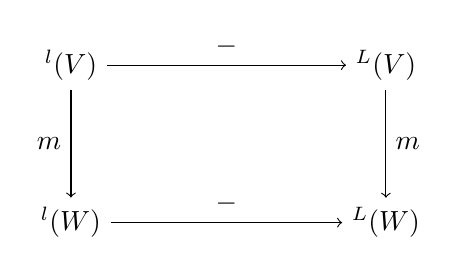
\begin{tikzpicture}[xscale=4,yscale=2]
  \node (00) at (0,0) {$\Exp^l(V)$};
  \node (10) at (1,0) {$\Exp^L(\sem{V})$};
  \node (01) at (0,-1) {$\Exp^l(W)$};
  \node (11) at (1,-1) {$\Exp^L(\sem{W})$};

  \draw[->] (00) --node[above]{$\sem{-}$} (10);
  \draw[->] (01) --node[above]{$\sem{-}$} (11);
  \draw[->] (00) --node[left]{$\ov{m}$} (01);
  \draw[->] (10) --node[right]{$\ov{\sem{m}}$} (11);
\end{tikzpicture}
\end{center}
\end{frame}

\begin{frame}\frametitle{Substitution Theorem for translation/substitutions}
Given:
\begin{itemize}
\item formal systems $l$, $L$ with contexts and substitutions
\item a compositional translation $\sem{-}:l\to L$
\item an $l$-vocabulary $V$ and a $V$-substitution $\gamma:\Gamma\to\Delta$
\end{itemize}

\[\sem{E[\gamma]}\;\; = \;\; \sem{E}[\sem{\gamma}]\]

\begin{center}
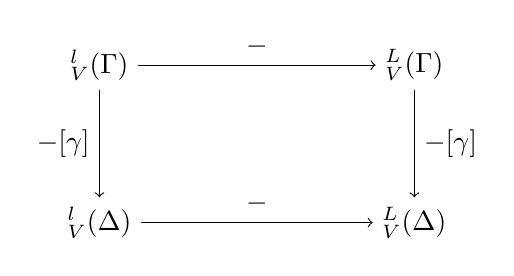
\begin{tikzpicture}[xscale=4,yscale=2]
  \node (00) at (0,0) {$\Exp^l_V(\Gamma)$};
  \node (10) at (1,0) {$\Exp^L_{\sem{V}}(\sem{\Gamma})$};
  \node (01) at (0,-1) {$\Exp^l_V(\Delta)$};
  \node (11) at (1,-1) {$\Exp^L_{\sem{V}}(\sem{\Delta})$};

  \draw[->] (00) --node[above]{$\sem{-}$} (10);
  \draw[->] (01) --node[above]{$\sem{-}$} (11);
  \draw[->] (00) --node[left]{$-[\gamma]$} (01);
  \draw[->] (10) --node[right]{$-[\sem{\gamma}]$} (11);
\end{tikzpicture}
\end{center}
\end{frame}

\begin{frame}\frametitle{Substitution Theorem for morphisms/substitutions}
Given:
\begin{itemize}
\item formal system $l$ with morphisms and contexts and substitutions
\item a morphism $m:V\to W$
\item a $V$-substitution $\gamma:\Gamma\to\Delta$
\end{itemize}

\[\ov{m}(E[\gamma])\;\; = \;\; \ov{m}(E)[\ov{m}(\gamma)]\]

\begin{center}
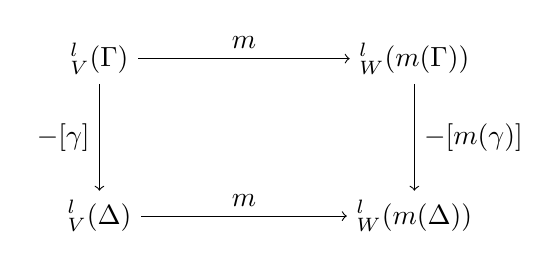
\begin{tikzpicture}[xscale=4,yscale=2]
  \node (00) at (0,0) {$\Exp^l_V(\Gamma)$};
  \node (10) at (1,0) {$\Exp^l_W(\ov{m}(\Gamma))$};
  \node (01) at (0,-1) {$\Exp^l_V(\Delta)$};
  \node (11) at (1,-1) {$\Exp^l_W(\ov{m}(\Delta))$};

  \draw[->] (00) --node[above]{$\ov{m}$} (10);
  \draw[->] (01) --node[above]{$\ov{m}$} (11);
  \draw[->] (00) --node[left]{$-[\gamma]$} (01);
  \draw[->] (10) --node[right]{$-[\ov{m}(\gamma)]$} (11);
\end{tikzpicture}
\end{center}
\end{frame}

\begin{frame}\frametitle{Substitution Theorem for the general case}
The previous cases can be seen as faces of a cube where corners are triples of language, vocabulary, context.

In general, we have
\begin{itemize}
\item formal systems $l$, $L$ with morphisms and contexts and substitutions and a compositional translation $\sem{-}:l\to L$
\item $l$-vocabularies $V$, $W$, and an $l$-morphism $m:V\to W$
\item $V$-contexts $\Gamma$, $\Delta$, and a $V$-substitution $\gamma:\Gamma\to\Delta$
\end{itemize}
and all $6$ orders of applying $\sem{-}$, $\ov{m}$, and $\gamma$ yield equal results.
\end{frame}



%\begin{frame}\frametitle{Example: Relative Computational Semantics for BOL}
%Scala, SQL semantics evaluates
%\begin{itemize}
%\item concept $c$ to
%\begin{itemize}
%\item SQL: table of individuals
% \lec{result of running query $\sem{c}$}
%\item Scala: hashset of individuals
% \lec{result of running program $\sem{c}$}
%\end{itemize}
%\item propositions to booleans \lec{accordingly}
%\end{itemize}
%
%Technically, results not in image of $\sem{-}$\\
%Fix: add productions for all values
%\begin{commgrammar}
%\gprod{F}{\true\bnfalt \false}{truth values}\\
%\gprod{C}{\{I,\ldots,I\}}{finite concepts}
%\end{commgrammar}
%\end{frame}

%
%\begin{frame}\frametitle{Equivalence of BOL Semantics}
%Now $5$ semantics for BOL
%\begin{itemize}
%\item absolute deductive via calculus
%\item relative deductive via SFOL
%\item relative computational via Scala
%\item relative concrete via SQL
%\item relative narrative via English
%\end{itemize}
%Moreover, these are interdefinable.
%\glec{e.g., Scala translation also induces deductive semantics}
%
%Can compare equivalence
%\begin{itemize}
%\item for every pair of semantics
%\item for every kind of equivalence (deductive, concrete, computational)
%\end{itemize}
%Question: Which of them hold?
%\end{frame}
%
%\begin{frame}\frametitle{Questions}
%For example, consider:
%\begin{itemize}
%\item Are the absolute semantics and the Scala semantics deductively equivalent?
%\item Assuming BOL and SQL have the base types and values:
%Are the absolute semantics and the SQL semantics concretely equivalent?
%\end{itemize}
%\end{frame}
%
%
%\begin{frame}\frametitle{Computational Semantics of BOL}
%Are these two BOL semantics deductively equivalent
%\begin{itemize}
%\item absolute deductive semantics 
%\item relative deductive semantics via translation $\sem{-}$ to Scala
%\end{itemize}
%
%\only<1>{
%Soundness: $\vdash^{BOL}_V f$ implies $\vdash^{Scala}_{\sem{V}}\sem{f}\rewrites \true$
%\begin{itemize}
%\item Problem: Absolute semantics performs consequence closure, e.g.,
%\begin{itemize}
%\item transitivity of $\sqsubseteq$
%\item relationship between $\sqsubseteq$ and $\isa$
%\end{itemize}
%\item Scala semantics does so only if we explicitly implemented it
%\glec{we didn't}
%\glec{same problem for SQL semantics}
%\end{itemize}
%}
%
%\only<2>{
%Completness: $\vdash^{BOL}_V f$ implied by $\vdash^{Scala}_{\sem{V}}\sem{f}\rewrites \true$
%\begin{itemize}
% \item absolute semantics leaves closed world optional
% \item Scala uses closed worlds
%  \glec{e.g., used to compute $c\sqsubseteq d$ by checking all individuals} 
% \item complete only if we add induction rule
%\end{itemize}
%}
%\end{frame}
